\chapterimage{/4/head4.png} % Chapter heading image
\chapter{Storia Cronologica dell'Universo}\label{5:ch}

Non ci si avventurerà nella selva oscura della teoria GUT, ma verranno soltanto citati graficamente i fenomini-chiave e i principali periodi che caratterizzano le primissime fasi di vita del nostro universo. A partire dal tempo di Plank, $t_P=10^{-43}$ s, gli effetti quantistici diminuiscono col passare degli istanti, ma leptoni e adroni sono ancora la stessa cosa. Per questo motivo in questa fase può essere violata la conservazione del numero barionico, ma essendo in equilibrio si ha: $n_b = n_{\overbar{b}}$ e qualunque eventuale eccesso può essere cancellato da reazioni che violano il numero barionico. La transizione GUT è l'unico momento in cui può essersi formata l'anisotropia di 1 parte su $10^8$ barioni (i modelli di bariogenesi faticano ancora a trovare un valore così piccolo). Inoltre in questi istanti si formano le cariche, tra cui i monopoli magnetici. Durante la fase intermedia successiva, che dura $10^{26}$ secondi, la temperatura cala di $12$ dex e alla fine si ha $R_H = 1$ cm. La fisica delle particelle fatica a trovare candidati per questo range di temperature, per questo il periodo viene definito \textit{deserto di particelle}. La seconda transizione importante è quella elettrodebole, durante la quale i leptoni e il neutrino possono prendere massa. Infine all'ultima transizione quark-adroni si ha $R_H = 1$ km. Da questo punto si introducono i modelli inflazionari.
\begin{figure}[H]
    \centering
    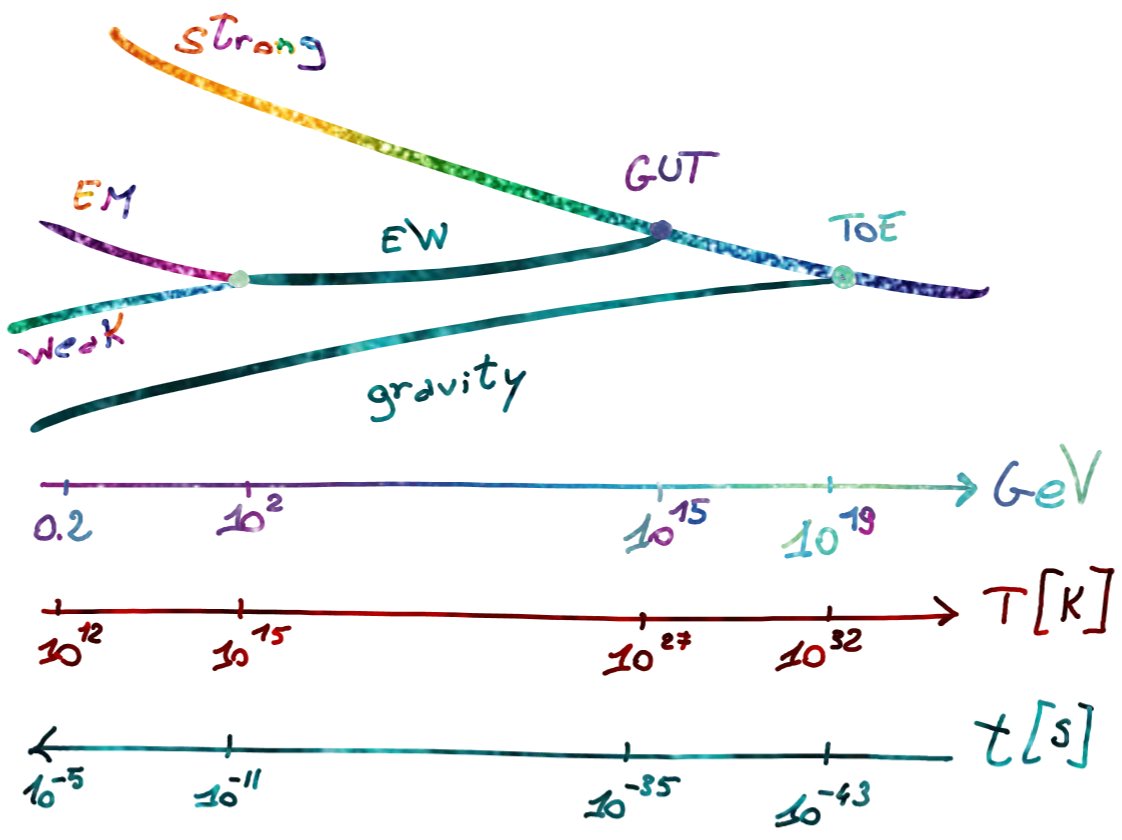
\includegraphics[width=.55 \textwidth]{Pictures/5/fasiprimordiali.png}
    \label{fig:4}
\end{figure}


\section{Modello Guth (\textit{old inflation})}